\documentclass{article}

\usepackage{titlesec}
\usepackage{longtable}
\usepackage{array} % for defining a new column type
\usepackage{varwidth} %for the varwidth minipage environment
\usepackage{color, colortbl}
\usepackage{caption}
\usepackage{subfigure}
\usepackage{filecontents}
\usepackage[section]{placeins}
\usepackage{float}
\usepackage{lscape}

\definecolor{Gray}{gray}{0.9}

\usepackage{pgf-umlsd}
\usepackage{pgf-umlcd}

\usepackage[latin1]{inputenc}
\usepackage{tikz}
\usetikzlibrary{shapes,arrows}

\newcommand{\sectionbreak}{\clearpage}

\begin{document}


\tikzstyle{decision} = [diamond, draw, fill=blue!20, 
    text width=4.5em, text badly centered, node distance=3cm, inner sep=0pt]
\tikzstyle{block} = [rectangle, draw, fill=blue!20, 
    text width=5em, text centered, rounded corners, minimum height=4em]
\tikzstyle{line} = [draw, -latex']
\tikzstyle{cloud} = [draw, ellipse,fill=red!20, node distance=3cm,
    minimum height=2em]

\newcolumntype{M}{>{\begin{varwidth}{4cm}}l<{\end{varwidth}}} %M is for Maximal column

\begin{titlepage}
	\Huge{Bitcode Assignment 3}
\end{titlepage}


\section{Design Patterns}
Using design patterns in software project is a good practice. It helps to make your software understandable, sustainable and expendable. We have chosen two design patterns and implemented them in our existing code, the state pattern and the strategy pattern.

\subsection{The State Design Pattern}
why? tbd

\subsubsection{State Class Diagram}
tbd

\subsubsection{State Sequence Diagram}
tbd

\subsection{The Strategy Design Pattern}
why? tbd

\subsubsection{Strategy Class Diagram}
tbd

\subsubsection{Strategy Sequence Diagram} 
tbd

\newpage
\section{Defensive Programming}
In the previous assignments it was required to use a game configuration file for initializing variables using a provided library. However, the provided library introduced bugs in the game. 
\paragraph{} To solve the bugs we have created a wrapper class (CameConfig) around the library's API that catches all the bugs and checks if the variables are within limits. This means that for every different API call we created a method in the GameConfig class. In the sequence diagram below is shown how the wrapper class works.

\begin{figure}[H]
	\centering
	\begin{sequencediagram}
		\newthread{A}{:Launcher}{}
		\newthread{B}{:GameConfig}{}
		\newthread{C}{:DefProAPI}{}
		\begin{call}{A}{getString()}{B}{}
			\begin{call}{B}{getStringValue()}{C}{}
			\end{call}
		\end{call}
	\end{sequencediagram}
\end{figure}

\paragraph{} In every method in the CameConfig class that implements the API checks are build in to verify the data that is returned by the API. Also if the API throws an exception it is catched in the method. If an exception occurs or the data returned by the API is not within the defined boundaries the method will return the defined default value. The flowchart below shows how the method getString() is implemented.

\begin{tikzpicture}[node distance = 2cm, auto]
    % Place nodes
    \node [block] (defpro) {getString ValueOf()};
    \node [cloud, left of=defpro] (start) {getString()};
	\node [decision, below of=defpro] (exception) {no exception?};
	\node [decision, below of=exception] (limit) {within limits?};
	\node [decision, below of=limit] (alpha) {is alphabetic?};
	\node [block, left of=alpha, node distance=3cm] (default) {return default value};
    \node [block, right of=alpha, node distance=3cm] (config) {return config value};
    
    \path [line,dashed] (start) -- (defpro);
    \path [line] (defpro) -- (exception);
	\path [line] (exception) -- node {yes}(limit);
	\path [line] (limit) -- node {yes}(alpha);
	\path [line] (alpha) -- node {no}(default);
	\path [line] (alpha) -- node {yes}(config);
	
	\path [line] (exception) -| node {no}(default);
	\path [line] (limit) -| node {no}(default);
    
\end{tikzpicture}  

\paragraph{} In this particular example the following conditions makes the method return the defined default value.
\begin{itemize}
	\item If the library thorows an exception.
	\item If the amount of characters in the sting is less or more then expected.
	\item If the string is not alphabetic.
\end{itemize}

\section{Selectable Difficulty}
One way of making the game more competitive is to implement selectable difficulty. The idea is that the user can select a desired difficultly between easy, normal and hard before the game starts. The selected level of difficulty will noticeably influence the difficulty of the game.   

\subsection{Requirements}
The requirements are ordered by the MoSCoW model.

\paragraph{Must Have:}
\begin{itemize}
	\item The game must have three levels of difficulty, easy, normal and hard.
	\item The player must be able to select the desired difficulty befor the game starts.
	\item The game must have a start screen.
\end{itemize}

\paragraph{Should Have:}
\begin{itemize}
	\item The player should get more points when removing a tile or a background tile when the game is more difficult.
\end{itemize}


\paragraph{Could Have:}
\begin{itemize}
	\item Higher difficulty could mean that the player should find four of the same tiles on a row.
	\item Higher difficulty could mean that the player has less moves to remove all background tiles.
	\item Higher difficulty could mean that there are more background tiles. 
	\item Lower difficulty could mean six different tiles instead of 7 tiles.
\end{itemize}


\newpage
\subsection{Software Design}
The figure below shows the class diagram of the implementation.
\begin{figure}[H]
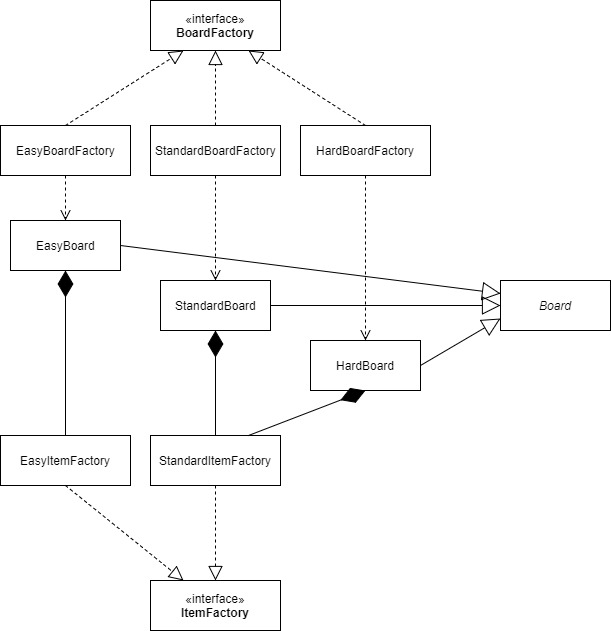
\includegraphics[scale=0.55]{Images/DifficultiesClassDiagram.jpg}
\end{figure}





\end{document}






